\documentclass[runningheads]{llncs}
\usepackage{graphicx}
\usepackage[utf8]{inputenc}
\usepackage[spanish]{babel}

\begin{document}


\title{metR - An R package for meteorological fields}

%\titlerunning{Abbreviated paper title}
% If the paper title is too long for the running head, you can set
% an abbreviated paper title here
%
\author{Elio Campitelli\inst{1}}

%
\authorrunning{E. Campitelli}
% First names are abbreviated in the running head.
% If there are more than two authors, 'et al.' is used.
%
\institute{Centro de Investigaciones del Mar y la Atmósfera \\
    \email{eliocampitelli@cima.fcen.uba.ar}\\
    %\url{http://www.springer.com/gp/computer-science/lncs}
    }
%
\maketitle              % typeset the header of the contribution
%
\begin{abstract}
\keywords{meteorología  \and data \and Another keyword.}
\end{abstract}


\section{Introducción}\label{introduccion}

Gran parte de la investigación en ciencias de la atmósfera consiste en
el análisis y visualización de datos.

Un software de visualización de datos meteorológicos y oceanográficos
muy utilizado es GrADs (Grid Analysis and Display System) el cual
permite leer y graficar campos escalares y vectoriales con gran
facilidad. Sin emabrgo, su lenguaje de scripting es muy limitado, carece
de capacidades estadísticas nativas y no existen gran cantidad de
extensiones que las implementen. R, en cambio, posee implementaciones de
virtualmente cualquier tratamiento estadístico usado en ciencias de la
atmósfera y el paquete \texttt{raster} que permite leer y graficar datos
geográficos con relativa facilidad, pero por su naturaleza los datos
quedan opacados detrás de una estructura complicada que no es fácil
hacer interactuar con otros paquetes; en particular, no es posible
graficar utilizando \texttt{ggplot2}.

La finalidad de \texttt{metR} es proveer facilidades en la lectura,
manejo y visualización de datos meteorológicos en R utilizando
estructuras comunes soportadas por la mayoría de los paquetes, de manera
de poder beneficiarse de las implementaciones de la comunidad. Hace
fuerte uso de \texttt{data.table} por su eficiencia en memoria y
velocidad dada la gran cantidad de datos que suelen usarse en
meteorología, y en \texttt{ggplot2} por su flexibilidad y facilidad en
la creación de gráficos.

\section{Ejemplo}\label{ejemplo}

Como ejemplo, se usan los datos de altura geopotencial media mensual en
el nivel de 700hPa entre 1990 y 2000, que vienen incluidos en
\texttt{metR}.

Se calculan las anomalías temporales para cada puntos de grilla y
calcular el campo asociado a la primera componente principal para cada
mes. Finalmente, se calcula el viento geostrófico correspondiente a ese
campo. Todo este proceso toma unas pocas líneas de código y se integra
sin esfuerzo en el \emph{workflow} de \texttt{data.table}.

\begin{Shaded}
\begin{Highlighting}[]
\NormalTok{geopotential[, gh.t }\OperatorTok{:}\ErrorTok{=}\StringTok{ }\KeywordTok{Anomaly}\NormalTok{(gh), by =}\StringTok{ }\NormalTok{.(lon, lat, }\KeywordTok{month}\NormalTok{(date))]}
\NormalTok{geopotential[, gh.t.w }\OperatorTok{:}\ErrorTok{=}\StringTok{ }\NormalTok{gh.t}\OperatorTok{*}\KeywordTok{sqrt}\NormalTok{(}\KeywordTok{cos}\NormalTok{(lat}\OperatorTok{*}\NormalTok{pi}\OperatorTok{/}\DecValTok{180}\NormalTok{))]}
\NormalTok{eof <-}\StringTok{ }\NormalTok{geopotential[, }\KeywordTok{EOF}\NormalTok{(gh.t.w }\OperatorTok{~}\StringTok{ }\NormalTok{date }\OperatorTok{|}\StringTok{ }\NormalTok{lon }\OperatorTok{+}\StringTok{ }\NormalTok{lat, }\DataTypeTok{n =} \DecValTok{1}\NormalTok{)}\OperatorTok{$}\NormalTok{right, by =}\StringTok{ }\NormalTok{.(}\KeywordTok{month}\NormalTok{(date))]}
\NormalTok{eof[, }\KeywordTok{c}\NormalTok{(}\StringTok{"u"}\NormalTok{, }\StringTok{"v"}\NormalTok{) }\OperatorTok{:}\ErrorTok{=}\StringTok{ }\KeywordTok{GeostrophicWind}\NormalTok{(gh.t.w, lon, lat), by =}\StringTok{ }\NormalTok{.(month)]}
\end{Highlighting}
\end{Shaded}

Luego, se grafica el campo de geopotencial con contornos llenos de
manera que haya una relación uno a uno entre los niveles graficados y
los señalados en la escala de colores. El campo de movimiento, por su
parte, se grafica con líneas de corriente.

\begin{Shaded}
\begin{Highlighting}[]
\NormalTok{binwidth <-}\StringTok{ }\FloatTok{0.01}
\KeywordTok{ggplot}\NormalTok{(eof[month }\OperatorTok\StringTok{ }\DecValTok{1}\OperatorTok{:}\DecValTok{2}\NormalTok{], }\KeywordTok{aes}\NormalTok{(lon, lat)) }\OperatorTok{+}
\StringTok{   }\KeywordTok{geom_contour_fill}\NormalTok{(}\KeywordTok{aes}\NormalTok{(}\DataTypeTok{z =}\NormalTok{ gh.t.w), }\DataTypeTok{circular =} \StringTok{"x"}\NormalTok{, }\DataTypeTok{breaks =} \KeywordTok{AnchorBreaks}\NormalTok{(}\DecValTok{0}\NormalTok{, binwidth, }\DecValTok{0}\NormalTok{)) }\OperatorTok{+}
\StringTok{   }\KeywordTok{geom_streamline}\NormalTok{(}\KeywordTok{aes}\NormalTok{(}\DataTypeTok{dx =} \KeywordTok{dlon}\NormalTok{(u, lat), }\DataTypeTok{dy =} \KeywordTok{dlat}\NormalTok{(v)), }\DataTypeTok{L =} \DecValTok{30}\NormalTok{, }\DataTypeTok{skip =} \DecValTok{2}\NormalTok{) }\OperatorTok{+}
\StringTok{   }\NormalTok{geom_map }\OperatorTok{+}
\StringTok{   }\KeywordTok{scale_fill_divergent}\NormalTok{(}\DataTypeTok{breaks =} \KeywordTok{AnchorBreaks}\NormalTok{(}\DecValTok{0}\NormalTok{, binwidth, }\DecValTok{0}\NormalTok{), }\DataTypeTok{guide =} \StringTok{"colorstrip"}\NormalTok{, }\DataTypeTok{name =} \StringTok{""}\NormalTok{) }\OperatorTok{+}
\StringTok{   }\KeywordTok{scale_y_latitude}\NormalTok{(}\DataTypeTok{ticks =} \DecValTok{15}\NormalTok{) }\OperatorTok{+}
\StringTok{   }\KeywordTok{scale_x_longitude}\NormalTok{() }\OperatorTok{+}
\StringTok{   }\KeywordTok{coord_quickmap}\NormalTok{(}\DataTypeTok{xlim =} \KeywordTok{c}\NormalTok{(}\DecValTok{0}\NormalTok{, }\DecValTok{360}\NormalTok{), }\DataTypeTok{ylim =} \KeywordTok{c}\NormalTok{(}\OperatorTok{-}\DecValTok{90}\NormalTok{, }\OperatorTok{-}\DecValTok{20}\NormalTok{)) }\OperatorTok{+}
\StringTok{   }\KeywordTok{facet_wrap}\NormalTok{(}\OperatorTok{~}\StringTok{ }\NormalTok{month, }\DataTypeTok{ncol =} \DecValTok{1}\NormalTok{, }
              \DataTypeTok{labeller =} \KeywordTok{labeller}\NormalTok{(}\DataTypeTok{month =} \KeywordTok{setNames}\NormalTok{(month.abb, }\KeywordTok{as.character}\NormalTok{(}\DecValTok{1}\OperatorTok{:}\DecValTok{12}\NormalTok{)))) }\OperatorTok{+}
\StringTok{   }\KeywordTok{theme_minimal}\NormalTok{() }\OperatorTok{+}\StringTok{ }\KeywordTok{theme_field}\NormalTok{()}
\end{Highlighting}
\end{Shaded}

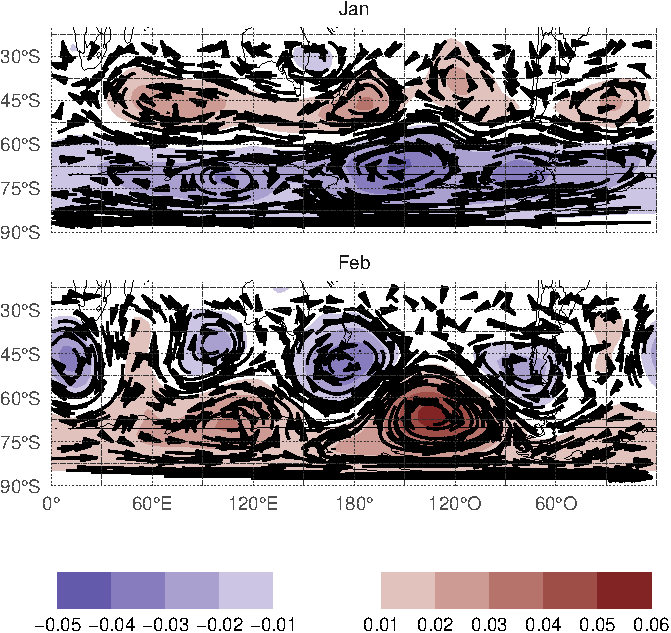
\includegraphics{abstract_files/figure-latex/unnamed-chunk-3-1.pdf}

\section{Limitaciones}\label{limitaciones}

El uso de \texttt{data.table}s para el manejo de datos implica una
importante limitación para \texttt{metR}. Muchas aplicaciones
meteorológicas hacen uso de cantidades de datos que resultan imposibles
cargar en memoria RAM en la mayoría de las computadoras personales.
\texttt{metR} tampoco puede manejar campos que no se encuentren en en
grillas regulares o en grillas proyectadas. En ambos casos paquetes como
\texttt{raster} y \texttt{rasterVis} son indispensables.

\texttt{metR} está en estado experimental y de activo desarrollo, tanto
en crecimiento de funcionalidad como en refinamiento de interfaces y
corrección de errores. Como todo proyecto de código abierto, es deseable
además que a medida que sea adoptado por la comunidad, surgan nuevos
casos de uso que incentiven su evolución más allá de las necesidades
personales de un sólo desarrollador.


\end{document}
